% Part: sets-functions-relations
% Chapter: infinite
% Section: hilberts-hotel
%
\documentclass[../../../include/open-logic-section]{subfiles}

\begin{document}

\olfileid{sfr}{infinite}{hilbert}
\olsection{हिल्बर्ट यांचे हॉटेल}

नैसर्गिक संख्यांचा संच स्पष्टपणे अनंत आहे. म्हणून, नैसर्गिक संख्या
स्वतःच \emph{आयत्या गृहीत धरायच्या} नसतील, तर नैसर्गिक संख्यांचा उल्लेख
न करता अनंत संचाचे वैशिष्ट्य सांगणे ही आपली पहिली पायरी असली पाहिजे.
सन 1924 मधील एका व्याख्यानात हिल्बर्ट यांनी मांडलेला पुढील दृष्टिकोन
सुबक आहे. ते आपल्याला अशी कल्पना करायला सांगतात:
\begin{quote}
[\ldots] सांत संख्येने खोल्या असलेले एक हॉटेल. या सर्व खोल्यांपैकी
प्रत्येक खोलीत नेमका एक पाहुणा असावा. आता पाहुण्यांनी कशाही प्रकारे
आपापल्या खोल्या बदलल्या, [पण] प्रत्येक खोलीत अजूनही एकापेक्षा अधिक
व्यक्ती राहणार नाही अशा रीतीने, तर एकही खोली मोकळी होणार नाही आणि
हॉटेलमालकाला या मार्गाने नव्याने येणाऱ्या पाहुण्यासाठी नवी जागा निर्माण
करता येणार नाही [\ldots
\textparagraph \ldots]

आता हॉटेलमध्ये $1$, $2$, $3$, $4$, $5$, \dots अशा क्रमांकांच्या अनंत
खोल्या असतील आणि प्रत्येक खोलीत नेमका एक पाहुणा असेल, असे आपण ठरवू.
नवा पाहुणा येताच मालकाने प्रत्येक जुन्या पाहुण्याला त्याच्या खोलीच्या
क्रमांकापेक्षा एकाने मोठा क्रमांक असलेल्या खोलीत हलवायचे असते; मग नव्याने
आलेल्या पाहुण्यासाठी खोली~$1$ मोकळी होईल.
	\begin{center}
		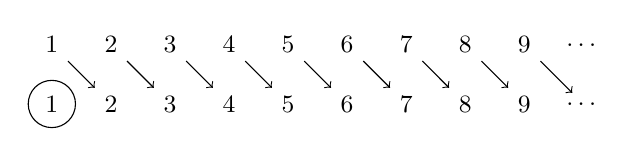
\begin{tikzpicture}[scale = .75]
		\foreach \x in {1, 2, 3, 4, 5, 6, 7, 8, 9}
		{
			\node (\x a) at (\x, 1) {\small{\x}};
			\node (\x b) at (\x, 2) {\small{\x}};
		}
		\node (dotsa) at (10, 1) {\small{\ldots}};
		\node (dotsb) at (10, 2) {\small{\ldots}};
		\draw[->] (1b)--(2a);
		\draw[->] (2b)--(3a);
		\draw[->] (3b)--(4a);
		\draw[->] (4b)--(5a);
		\draw[->] (5b)--(6a);
		\draw[->] (6b)--(7a);
		\draw[->] (7b)--(8a);
		\draw[->] (8b)--(9a);
		\draw[->] (9b)--(dotsa);
		\draw (1,1) circle (.4);
		\end{tikzpicture}
	\end{center}
	(\citealt[730]{EwaldSieg2013} मध्ये प्रकाशित; अनुवाद आमचा)
\end{quote}
निर्णायक मुद्दा असा की हिल्बर्ट यांच्या हॉटेलमध्ये अनंत खोल्या आहेत;
आणि असे म्हणण्याचा अर्थ काय, याची व्याख्या म्हणून आपण त्यांचे स्पष्टीकरण
घेऊ शकतो. खरे तर हाच डेडेकिंड यांचा दृष्टिकोन होता (अर्थातच येथे फार
मोठा कालविपर्यास करून तो मांडला आहे; डेडेकिंड यांची व्याख्या
\citeyear{Dedekind1888} मधील आहे):

\begin{defn}\ollabel{defn:DedekindInfinite}
संच $A$ हा \emph{डेडेकिंड-अनंत} असतो जर आणि तरच $A$ पासून~$A$ च्या
एखाद्या उचित उपसंचाकडे !!a{injection} असते. म्हणजे, असा काही $o \in A$
आणि !!a{injection} $f \colon A \to A$ असतात की $o \notin \ran{f}$.
\end{defn}

\end{document}
